\documentclass[border=3pt]{standalone}
\usepackage{tikz}
\usetikzlibrary{arrows.meta,calc,positioning}
\tikzset{bus/.style={{Stealth[length=5pt]}-{Stealth[length=5pt]}, thick},
  blk/.style={draw, thick, font=\sffamily\small, align=center}}
\begin{document}
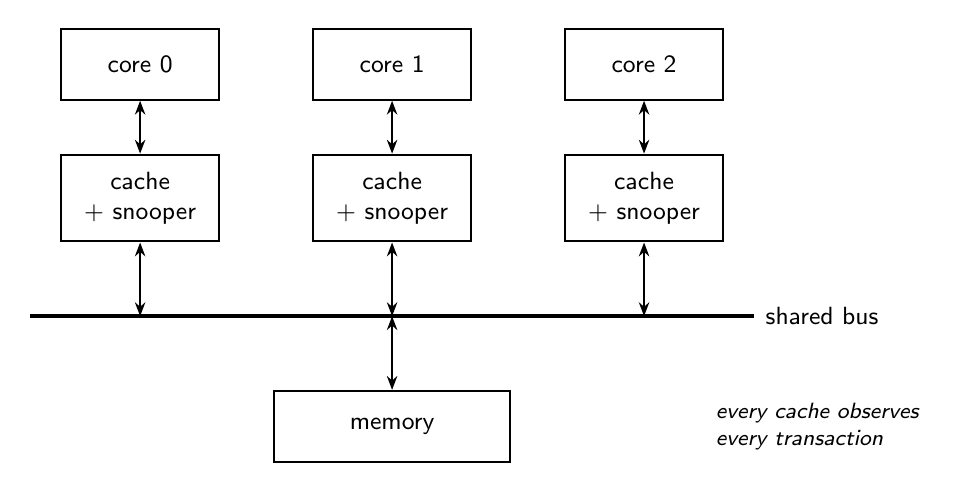
\begin{tikzpicture}[font=\sffamily\small]
  \foreach \i/\x in {0/0, 1/3.2, 2/6.4}{
    \node[blk, minimum width=20mm, minimum height=9mm] (c\i) at (\x,2.6) {core \i};
    \node[blk, minimum width=20mm, minimum height=11mm] (l\i) at (\x,0.9) {cache\\+ snooper};
    \draw[bus] (c\i.south) -- (l\i.north);
    \draw[bus] (l\i.south) -- (\x,-0.6);}
  % shared bus
  \draw[ultra thick] (-1.4,-0.6) -- (7.8,-0.6) node[right, font=\sffamily\small]{shared bus};
  % memory
  \node[blk, minimum width=30mm, minimum height=9mm] (mem) at (3.2,-2.0) {memory};
  \draw[bus] (mem.north) -- (3.2,-0.6);
  \node[font=\sffamily\footnotesize\itshape, align=left] at (8.6,-2.0) {every cache observes\\every transaction};
\end{tikzpicture}
\end{document}
